\documentclass[a4paper]{article}

\usepackage{color}
\usepackage{url}
\usepackage[utf8]{inputenc}
\usepackage[T2A]{fontenc}
\usepackage{graphicx}

\usepackage{pgfplots}
\pgfplotsset{compat=1.7}

\usepackage[english,serbian c]{babel}
\usepackage[unicode]{hyperref}
\hypersetup{colorlinks,citecolor=green,filecolor=green,linkcolor=blue,urlcolor=blue}

\begin{document}

\title{Паметне куће: Колико су безбедни Ваши подаци?\\ \small{Семинарски рад у оквиру курса\\Рачунарство и друштво\\Математички факултет}}

\author{Тамара Ђукић\\ tamarazdjukic@gmail.com}
\date{24.~мај 2022.}
\maketitle

\begin{center}
    \textbf{Апстракт}
\end{center}
\hspace{0.5cm}Брз технолошки напредак, све већа дигитализација и све већи токови података су допринели настанку и доста великом коришћењу паметних кућа. Идеја о
повезаној „паметној“\space кући је све више актуелнија и примамљивија него икада. Али шта тачно значи паметна кућа? Где леже корени ове технологије?
Које су користи и ризици? Како ће изгледати паметна кућа у будућности? На нека од ових питања ћемо одговорити у наставку текста.

\newpage

\tableofcontents

\newpage
\section{Увод}
Паметна кућа се односи на погодну кућну поставку где се уређаји могу аутоматски контролисати помоћу мобилног или другог умреженог уређаја са било ког места са поузданом интернет конекцијом.
Уређаји у паметној кући омогућавајући кориснику да на даљину контролише функције у својој кући као што су безбедносни приступ дому,
температура, осветљење, кућни биоскоп, итд.
\newline\newline
Уређаји паметне куће су међусобно повезани и може им се приступити преко једне централне тачке — паметног телефона, таблета, лаптопа, итд.
Систем је инсталиран на мобилном или другом умреженом уређају, и тада корисник може да креира временске распореде да одређене промене ступе на снагу.
\newline\newline
Паметне куће се могу реализовати као бежични или као жичани систем или оба. Бежичне системе је лакше инсталирати. Постављање бежичног система кућне аутоматизације са функцијама
као што су паметно осветљење, контрола климе и безбедност може коштати неколико хиљада долара, што га чини веома повољним. Са друге стране, жичани системи се сматрају поузданијим
и обично их је теже хаковати. Жичани систем може доста повећати вредност куће. Али постоји недостатак — прилично је скуп. Инсталирање луксузног и жичаног паметног система може
коштати власнике куће и до десетине хиљада долара.
\newline\newline
\begin{figure}[h!]
    \centering
    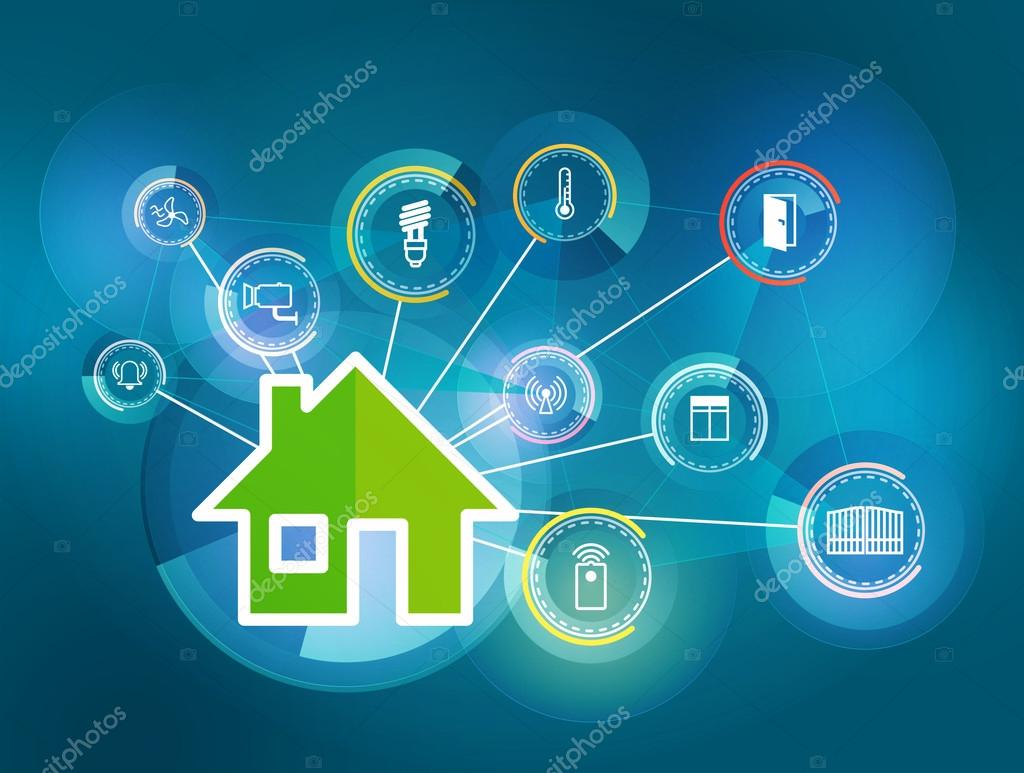
\includegraphics[width=0.6\textwidth]{Slike/smart_home.jpg}
    \caption{\label{fig:smart}Приказ паметне куће}
\end{figure}

\newpage
\section{Примери паметних уређаја}

\subsection{Паметан фрижидер}
Паметан фрижидер је уређај који има могућност повезивања на интернет. У зависности од фрижидера који одаберете и бренда, паметан фрижидер може понудити
неколико различитих практичних функција. Већина паметних фрижидера има могућност инсталирања апликације на мобилни телефон или друге уређаје како би омогућила
власнику да види ажурирања на свом фрижидеру и када није кући.
\newline\newline Неке карактеристике паметних фрижидера:
\begin{description}
    \item[Интерфејс екрана осетљивог на додир]
    Екран осетљив на додир на паметном фрижидеру се може користити за приступ разним функцијама притиском на екран. Новији модели могу имати велики екран
    са рачунарском снагом сличној оној на Вашем лаптопу. Такође, паметан фрижидер може да има уграђене звучнике који могу побољшати искуство коришћења.
    \item[Могућност повезивања на интернет]
    Паметан фрижидер има уграђен претраживач преко кога можемо да се повежемо на интернет и тражимо ствари које су нам потребне.
    \item[Унутрашња камера]
    Унутрашња камера нам може омогућити да видимо шта се налази унутар фрижидера без да га сваки пут отварамо. Предност унутрашње камере је смањење трошкова
    струје и храна се неће брзо кварити јер не улази топлота унутар фрижидера.
    \item[База рецепата]
    Имамо могућност чувања рецепата са интернета. Такође, фрижидер нам може читати кораке за неки рецепт или можемо пустити видео који објашњава кораке рецепта.
\end{description}

\subsection{Паметан усисивач}
Роботски усисивач, који се некад назива робовак (Robovac), је самостални усисивач који има ограничен систем за усисавање подова у комбинацији са сензорима
и роботским погонима са програмабилним контролерима и рутинама чишћења. Рани дизајни су укључивали ручно управљање путем даљинског управљача и режим
„самовожње“ који је омогућавао машини да самостално чисти без људске контроле. Неки дизајни користе окретне четке да би досегнули уске углове,
а неки укључују низ функција за (брисање, УВ стерилизација, итд.) чишћење заједно са функцијом усисавања. Новији модели користе вештачку интелигенцију
и дубоко учење за боље мапирање, идентификацију објеката и чишћење на основу догађаја.
\newline\newline Неке карактеристике паметних усисивача:
\begin{description}
    \item[Не морамо бити код куће да би кренуо да чисти]
    Имати роботски усисивач у свом животу значи да никада не морамо да одвајамо време за усисавање куће.
    Могу се програмирати да обилазе кућу док нисмо кући. Такође, можемо правити распореде према коме ће он сам кренути са своје станице да чисти
    и када нисмо код куће.
    \item[Самостално се пуни]
    Ови усисивачи се враћају на своју станицу ради поновног пуњења на крају сваког циклуса чишћења. Све док је њихова станица за пуњење укључена,
    никада не морамо да бринемо да ли ће се искључити током чишћења. Неки модели ће чак престати са чишћењем и вратити се на прикључну станицу
    ако открију да је батерија празна.
    \item[Флексибилни су за чишћење више врста површина]
    Роботски усисивачи су дизајнирани да се прилагођавају различитим површинама помоћу својих сензора који детектују промене на подним површинама.
    Можемо их пустити да се крећу свуда по нашој кући и са лакоћом се носе са променама површине.
    \item[Уграђени сензори који детектују прљавштину на одређеном месту]
    Роботски усисивачи имају уграђене сензоре који могу да открију који делови наше куће захтевају додатни рад, и усисивач ће након тога направити додатне
    пролазе преко тог подручја. Простори са великим прометом као што су ходници, улази и играонице добиће додатну пажњу која им је потребна да би били чисти.
\end{description}

\subsection{Паметна камера}
Паметне камере су типичне бежичне камере које раде више од снимања снимака и слика.
Ови уређаји имају додатне функције које нам могу помоћи да пратимо статус своје куће чак и када смо удаљени хиљадама километара.
\newline\newline Неке карактеристике паметне камере:
\begin{description}
    \item[Препознавање лица]
    Способност паметне камере за препознавање лица је једна од најзначајнијих предности инсталирања овог типа система сајбер безбедности.
    Помоћу овог уређаја можемо да будемо сигурни да добијамо само упозорења за стварне претње тако што ћемо отпремити слике своје породице
    и пријатеља или их означити као несумњиве на снимку.
    \item[Комуникација]
    Поред снимања слика, паметне камере су такође опремљене системима за аудио надзор који нам омогућавају да слушамо разговоре или
    пазимо на другу сумњиву буку у окружењу наше куће. Ако откријемо да се нешто лоше спрема у окружењу наше куће, можемо изненадити лопове
    тако што ћемо разговарати са њима и вербално их отерати како би помислили да сте у својој кући.
    \item[Детекција покрета]
    Ови уређаји су опремљени сензорима који детектују кретање и аутоматски се крећу ка извору кретања. Затим ради са функцијом препознавања лица да
    идентификује да ли је особа споља пријатељ или непријатељ и да нас упозори на њено присуство путем апликације за паметне телефоне.
    Такође има ноћни вид како би били сигурни да је наша кућа заштићена током целог дана.
\end{description}

\section{Дигитална и физичка безбедност}
Због недавног напретка технологиjе, све jе више савета о дигиталноj безбедности и о томе како остати безбедан на интернету. Да би се оваj
савет проширио на све слоjеве друштва, он ниjе намењен само деци, већ и одраслима. Технологиjа се стално развиjа и мења, па се као
резултат тога, дигиталне безбедносне претње могу jавити много брже него што су поjединци раниjе били навикнути када jе у питању лична
безбедност. Како ове претње нису физичке, постоjи ризик да буду схваћене мање озбиљно. Такође може доћи до неспоразума о томе шта jе
тачно претња. То jе делимично зато што поjединци могу пренети размишљања о физичкој сигурности на дигиталну сигурност, што их доводи
до погрешних очекивања о природи и последицама претњи са коjима се могу суочити.
\newline\newline
Међутим, важно jе дигиталну сигурност схватити jеднако озбиљно као и физичку. Ово jе посебно важно у контексту паметне куће.
Постоjе два примарна проблема при увођењу паметних уређаjа у дом:
\begin{itemize}
    \item Паметни уређаj jе безбедан, али ниjе сигуран - уређаj има неефикасну безбедност, на пример уређаj се може лако хаковати
    \item Паметни уређаj jе сигуран, али корисници немаjу контролу над подацима - корисницима се манипулише како би произвођачима
    омогућили приступ више података него што заиста су желели да поделе
\end{itemize}

\subsection{Паметни уређаj jе безбедан, али ниjе сигуран}
У случајевима када обезбеђена заштита није довољна, долази до проблема јер постоји разлика између размишљања корисника и
дизајнера уређаја. Корисници могу да верују овим уређајима зато што верују компанији која их производи, дизајнеру уређаја или зато
што нису свесни који подаци могу бити прикупљени. Ово се често компликује чињеницом да многи корисници претпостављају да су приватност и
безбедност синоними. Пошто подаци могу бити шифровани и безбедни од хакера, корисници могу претпоставити да су и поверљиви. То није нужно случај.
Нарочито код виртуелних помоћника који се активирају гласом (нпр. Amazon Alexa, Google Assistant), подаци се могу послати у центре за обраду или
чак ненамерно послати контактима \cite{1} \cite{2}. Када дође до таквих повреда, корисници се могу осећати изданим од стране ових уређаја и нерадо их
користе јер су изградили погрешно размишљање како уређај функционише.
\newline \newline
\emph{Раздвајање сигурности од погодности отежава просечном кориснику да одреди колико је сигуран одређени паметан уређај.}
\newline  \newline
Док су корисници упознати са обезбеђивањем физичке безбедности својих домова како би се заштитили, дигитална безбедност је релативно
нов концепт. Упркос едукацији о овој теми, корисници могу претпоставити да је уређај сигурнији него што јесте јер можда не узимају
у обзир како је сваки појединачни уређај повезан у њиховом дому, само да су уређаји у самом дому сигурни (да их је тешко украсти).
\newline  \newline
За већину корисника лакше је размишљати о физичкој безбедности него о дигиталној. У друштву је укорењено да власници кућа морају закључати
врата и прозоре како би спречили провале. Да би то урадили, могу да купе браве и аларме, које након постављања треба само да одржавају.
Ментални модел кућне сигурности jе да брава или алармни систем након куповине функционишу првенствено сами. Не треба га редовно
прегледавати или ажурирати и његово радно стање се лако може проверити погледом или додиром. Овај модел се може погрешно пренети на дигиталну безбедност.
\newline  \newline
Дигитална безбедност захтева сталну обазривост. Технологија је новија и стално се мења, тако да корисници паметних уређаја морају редовно да
проверавају да ли постоје безбедносни пропусти и ажурирања. Сваки уређај представља потенцијалну улазну тачку у кућну мрежу корисника, а
чињеница да су сви уређаји међусобно повезани значи да без довољно сигурности за сваки уређај, било који од њих може да се користи за приступ
информацијама које се налазе у другим деловима система. Ово је посебно проблем када корисници уводе паметне уређаје као што су усисивачи који се
раније нису сматрали безбедносном претњом. Ови уређаји су нови на тржишту, лако доступни и јефтини. Као резултат тога, они не морају нужно бити сигурни \cite{3}.

\subsection{Паметни уређаj jе сигуран, али корисници немаjу контролу над подацима}
Што се тиче другог питања, где паметан уређај може бити довољно безбедан, али се корисницима манипулише тако да произвођачима дозволе приступ
већем броју података него што желе да поделе. Увођење Опште уредбе о заштити података ОУЗП (General Data Protection Regulation GDPR)  је значајно помогло у регулисању контроле података,
посебно са приватношћу и сигурношћу \cite{4}. Добар је као метод контроле, посебно када омогућава корисницима да лако разумеју и контролишу своје податке.
Али у стварности, тешко је проценити колико су корисници свесни шта се дешава са њиховим подацима jер нису били у могућности или не разумеjу споразуме
коjе склапаjу са технолошким компаниjамa. ОУЗП је ставио велики терет на компаније да избришу и контролишу податке од којих су раније можда остваривале профит.
Није у њиховом интересу да дозволе корисницима да одустану од дељења својих личних података. Као резултат, прибегавају манипулацији корисницима како
би задржали своје податке.
\newline  \newline
Пример за то је компанија Фејсбук. Феjсбук jе већ неколико пута био ухваћен у прикупљању више података него што су корисници желели да поделе. Jедан од примера
jе да jе друштвена мрежа имала посебне аранжмане са више од 150 компаниjа за размену личних података своjих чланова. Речено jе да су већина њих друге технолошке компаниjе, 
али на списку су, између осталих, били и телефонски продавци, произвођачи аутомобила и медиjске организациjе. Феjсбук jе сада прибегао коришћењу
мрачних образаца корисничког искуства (UX) дизаjнирани тако да се придржавају ОУЗП-а и прикупља жељене податке. Тамни обрасци се дефинишу као ситуације у којима
„дизајнери користе своје знање о људском понашању (нпр. психологија) и жеље краjњих корисника да примене варљиву функционалност коjа ниjе у наjбољем интересу корисника“ \cite{5}.
Ово може бити у облику сакривања опциjа, додавања куповина или трошкова у последњем тренутку у корпе за куповину или употребе трик питања како би убедили кориснике да изаберу опциjе коjе иначе не би одабрали.
\newline  \newline
Употреба тамних образаца у UX дизаjну ниjе специфична само за Феjсбук. Тамни образци се лако имплементираjу и широко су распрострањени. У овом тренутку jедини начин борбе против њих, под
условом да корисници желе да користе услуге коjе пружа дизаjнер, jе да истраjу кроз опциjе читаjући пажљиво. Реално, многи корисници то неће учинити. Количина напора коjа jе потребна за борбу против
мрачних образаца за сваку веб страницу и услугу навела би многе кориснике да jедноставно заобиђу проблем и jедноставно кликну на „прихвати“. Томе се надаjу дизаjнери таквих интерфеjса.
\newline  \newline
Такође jе важно шта се дешава са прикупљеним подацима након што су прибављени од краjњег корисника. Без обзира да ли су подаци хаковани из несигурног система или уређаjа, као у првом случаjу, или jе
корисник изманипулисан да се одрекне више података него што jе намеравао, као у другом случаjу, краjњи резултат jе исти. Компаниjе коjе су их прикупиле могу поново користити изворне податке или их
продати трећим странама, а корисник нема контролу над овим, или у неким случаjевима чак и знање о томе. Све мере предострожности коjе се примењуjу од стране корисника могу само ограничити количину
прикупљених података. Ради одговараjуће сигурности и приватности, овим питањима се мораjу позабавити произвођачи паметних уређаjа и дизаjнери њихових интерфеjса.
\newline  \newline
У сценарију паметне куће, уместо да се мора ослањати на корисника да провери ниво безбедности паметних уређаја у свом дому, одговорност би требало да буде на произвођачу.
Дизаjн осетљив на вредност \cite{6} и уговорни дизаjн \cite{7} су начини да се корисници заштите од нежељених последица коришћења технологиjе. ОУЗП jе пример осигурања
да корисници података и произвођачи технологиjе дизаjном имплементираjу приватност, и на неки начин безбедност података. Оно што је, међутим,
потребно је ниво изнад овог. Потребан је етички дизајн који има на уму најбоље интересе корисника — избегавање тамних образаца и нуђење корисницима једноставних опција за
њихову безбедност.
\newline  \newline
Произвођачи мораjу ставити своjе кориснике на прво место и размотрити колико су њихови уређаjи сигурни. Уређаjи мораjу бити проjектовани имаjући у виду концепт
безбедности, како би се одговорило не само на питање „Може ли се неко идентификовати према овим подацима?“ али „Може ли се приступити овим подацима?“ и „Да ли
би корисник желео да подели ове податке?“. С обзиром на брзину и разноликост развоjа технологиjе, ниjе увек одмах jасно у коjе сврхе се наизглед безазлени
подаци могу користити у будућности. Неопходно jе разговарати и применити заштитне мере за заштиту корисника данас од потенциjалних претњи сутрашњице.

\section{Предности и мане паметне куће}

\subsection{Предности}
Паметне куће могу побољшати квалитет живота становника пружањем различитих услуга коjе му помажу у свакодневном животу.\newline\newline
Паметну кућу можемо да користимо за контролу окружења, она jе аутоматизована контролом неких уређаjа, попут оних коjи се
користе за осветљење и греjање, на основу различитих климатских услова. Новиjе технологиjе омогућаваjу праћење унутрашњег
окружења и активности корисника куће. Такође, могу независно да предузимаjу унапред програмиране радње ида управљаjу уређаjима према унапред дефинисаним обрасцима, независно или према захтевима корисника.
\newline\newline
\begin{description}
    \item[Потпуна контрола свих паметних уређаја са једним паметним уређајем]
    Ово значи да све док поседујемо паметан телефон или неки други паметан уређај и исправну интернет везу, већину уређаја у својој кући можемо контролисати са једне централне тачке.
    Ово нам даје потпуну контролу над нашом кућом и чак можемо да прилагодимо неколико подешавања у другим просторијама. Ако не желимо да идемо на неко место
    у кући да бисмо променили подешавања уређаја, можемо то да урадимо директно са свог места због софистицираног међусобног повезивања кућних апарата.
    \item[Обавештења у случају опасности]
    Паметне куће нам такође омогућавају да будемо обавештени у случају да постоје проблеми са нашом кућом. На пример, ако неко покуша да нам насилно уђе у кућу,
    добићемо обавештење на паметном телефону да је неовлашћена особа на нашем имању. Ово може помоћи да се ухвати лопов јер полиција може бити обавештена у реалном времену.
    \item[Уштеда времена]
    Пошто се са једним паметним уређајем могу контролисати сви паметни уређаји у нашој кући, вероватно ћемо на дуже време уштедети доста времена. Не морамо бити
    физички присутни кући да би кренула нека радња да се одвија. Потребно је само да дамо команду, и да наставимо да радимо нешто друго.
    Ово доста помаже људима који немају пуно времена.
\end{description}

\subsection{Мане}
Свака паметна кућа има доста добрих предности, али увек постоје мане које могу бити мање или више опасне.
\newline\newline
\begin{description}
    \item[Значајни трошкови инсталације]
    Један недостатак паметних кућа је то што могу бити прилично скупе.  Могу постојати значајни трошкови инсталације који могу износити више хиљада долара.
    У зависности од квалитета система, можда чак и нема ограничења и многи људи можда неће бити вољни да потроше ову количину новца на свој дом.
    Међутим, паметне куће нам такође могу уштедети новац на дуге стазе због уштеде енергије.
    \item[Поуздана интернет мрежа]
    Још једна мана паметних кућа је да им је потребна поуздана интернет веза да би исправно радиле. На пример, ако живимо у области где је интернет веза
    прилично лоша, можда ћемо имати озбиљне проблеме јер наши паметни кућни уређаји можда неће реаговати на начин на који желимо.
    \item[Брига о безбедности]
    Такође постоје и неки безбедносни проблеми повезани са технологијама паметних кућа. На пример, провалници би могли да хакују у наш систем паметне куће
    и отворе браву како би добили приступ нашем дому. Постоји могућност и да хакери упадну у наш систем и да нам украду све личне податке, или да виде када нисмо
    код куће да би могли да нам провале у кућу.
    \item[Беспомоћност ако технологија откаже]
    Наш технолошки напредак се може сматрати добрим јер може побољшати квалитет живота сваког од нас. Међутим, постоје и неки проблеми у вези са технологијом.
    На пример, можда ћемо бити прилично беспомоћни ако наша технологија паметне куће откаже. Пошто смо се увек ослањали на ову технологију да функционише
    и прилагодили своје понашање, можда ћемо се осећати изгубљено у случају да наша технологија паметне куће више неће радити.
    \item[Није погодна за све домове]
    Многи људи једноставно не воле идеју о паметном кући. Поготово старија генерација која је прилично скептична по питању тога. Пошто често чујемо
    о слабостима тих система који провалницима олакшавају улазак у нашу кућу, многи људи се могу уздржати од тих технологија паметних кућа и
    радије се ослањају на своје браве старе школе, чак и ако су те браве такође прилично несигурне.
\end{description}

\section{Статистике}
\begin{figure}[h!]
    \centering
    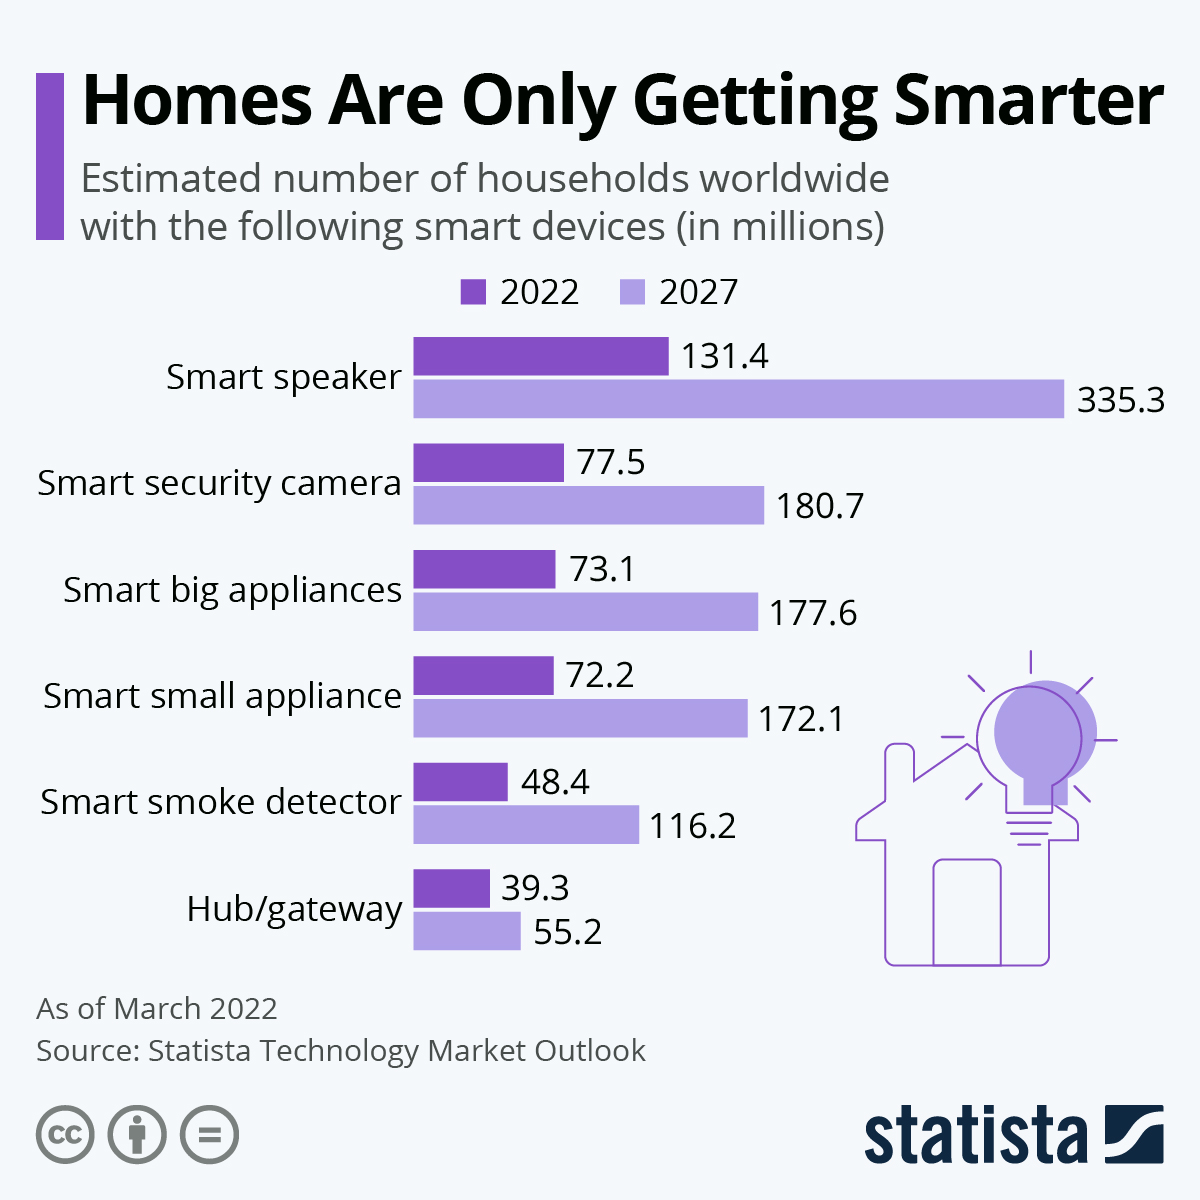
\includegraphics[width=0.6\textwidth]{Slike/statistics.png}
    \caption{\label{fig:stat}Статистике колико се данас користе паметни уређаји, и колико ће се користити у будућности}
\end{figure}

Неке занимљиве статистике:
\newline
\begin{itemize}
    \item До 2023. године, аутоматизација индустрије паметних кућа у америчким домовима биће 53,9\%
    \item Статистике показују да ће глобално тржиште паметних домова у 2022. години износити 53,5 милијарди долара
    \item Са обимом продаје од 23 милијарде долара, Сједињене Америчке Државе су највећи потрошач паметних технологија
    \item Пројекције показују да ће продор паметних звучника порасти за 55\% до 2022. године
    \item Процене показују да ће домаћинства потрошити 19,4 милијарде долара на куповину паметних безбедносних система
\end{itemize}

\section{Закључак}
У овом раду поменули смо неке од позитивних и негативних страна паметне куће. Паметне куће могу да нам живот учине много jедноставниjим,
поготово у областима здравствене неге, али долазе и са одређеним ризицима. Ако корисници са опрезом и разумевањем рукуjу паметним уређаjима,
негативне стране ће постати скоро занемарљиве. Када би посматрали паметне куће са стране етике утилитаризма правила, где jе нагласак на
укупноj срећи а не на томе шта се дешава поjединачним учесницима, дошли би до закључка да паметне куће доносе добро. Поготово ако узмемо
у обзир да део корисника и ниjе свестан свих (или jе одлучан да их игнорише) негативних аспеката паметних кућа.

\addcontentsline{toc}{section}{Литература}
\appendix

\iffalse
\bibliography{seminarski} 
\bibliographystyle{plain}
\fi

\begin{thebibliography}{seminarski}

\bibitem{1} L. Temple, \emph{“How new guidelines on smart devices will help protect consumers from being hacked,” Which? (online), 2018.}
\bibitem{2} A. Woodruff, S. E. Fox, S. Rousso-Schindler, and J. Warshaw, \emph{“A qualitative exploration of perceptions of algorithmic fairness,” in Proc. 36th ACM Conf. Hum. Factors Comput. Syst., pp. 1–14, 2018.}
\bibitem{3} A. Laughlin, \emph{“The cheap security cameras inviting hackers into your home,” Which? (online), 2019}
\bibitem{4} ICO,  \emph{“Guide  to  the  General  Data  Protection  Regulation  (GDPR),”}  Information Commissioner’s  Office  (online),  2018. [Online].  Available:
           https://ico.org.uk/for-оrganisations/guide-to-the-general-data-protection-regulation-gdpr/principles/lawfulness-fairness-and-transparency/. [Accessed: 27-Jun-2018].
\bibitem{5} C. M. Gray, Y. Kou, B. Battles, J. Hoggatt and A. L. Toombs \emph{“The Dark (Patterns) side of UX Design,” in Proc. 2018 CHI Conference on Human Factors in Computing Systems - CHI ’18, 2018, Apr. 2018, pp.1–14.}
\bibitem{6} B.  Friedman  and  P.  Kahn, \emph{“Value sensitive design: Theory and methods,” Univ. Washingt. Tech., pp. 1–8, Dec. 2002.}
\bibitem{7} J.  Pitt,  \emph{“Design contractualism for pervasive/affective computing,” Technol. Soc. Mag. IEEE, vol. 31, no. 4, pp. 22–29, 2012.}

\end{thebibliography}

\end{document}
